\documentclass[12pt]{article}
\usepackage[parfill]{parskip}
\usepackage{amsmath}
\usepackage{amssymb}
\usepackage{bm}
\usepackage{enumerate}
\usepackage{fancyvrb}
\usepackage[top=1in, bottom=1in, left=1in, right=1in]{geometry}
\usepackage{hyperref}
\hypersetup{
	colorlinks=true,
}
\usepackage{placeins}
\usepackage{tikz}
\usepackage{tikzsymbols}
\usepackage{todonotes}
\usepackage{bbm}
\usepackage{color}
\usepackage{enumitem}
\usepackage{xcolor}
\newcommand{\rmn}[1]{{\textcolor{blue}{\bf [{\sc rmn:} #1]}}}
\DeclareMathOperator*{\argmax}{arg\,max}
\usepackage{algorithmicx}
\usepackage{algorithm}
\usepackage{algpseudocode}
\usepackage{multirow}
\usepackage{rotating}

\usetikzlibrary{positioning,calc}
%%%%%%%%%
\usepackage[most]{tcolorbox}
\newtcolorbox[]{solution}[1][]{%
	breakable,
	enhanced,
	colback=white,
	title=Solution,
	#1
}
%%%%%%%%%%
\title{10-703 Deep Reinforcement Learning and Control\\
	Assignment 3\\
	Fall 2018 \\  
}
\author{ielshar \\ mharding}
\date{October 26, 2018}
\begin{document}
	
	\maketitle
	
	\section*{Problem 1: REINFORCE}
	\begin{enumerate}
		\item  Describe your implementation:
		\begin{itemize}
			\item Neural Network Architecture:  same as given in JSON file. No baseline was used.
			\item Learning rate: 0.001
			\item Discount factor $\gamma: 1$
		\end{itemize}
		\item 
		\begin{figure}[H]
			\begin{center} 
				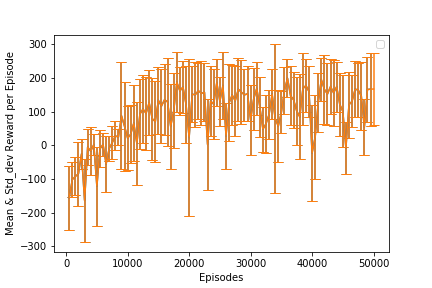
\includegraphics[scale=.73]{figures/Reinforce_LC_50.png}
			\end{center}
			\caption{REINFORCE Algorithm without baseline: learning curve - Every k=500 episodes the current policy is tested on 100 episodes. The plot shows the mean and standard deviation of each of this tests.  } 	\label{1}%
		\end{figure}
	\end{enumerate}
	
	Figure \ref{1} above shows that our agent was able to achieve a mean reward of 200  or slightly more or less at several points (after 36000 and 41500 episodes) throughout the training. Since no baseline was used in our REINFORCE algorithm one can see that the test results have a high variance. This is somehow expected though as the total return at the end of episode varies greatly from one sampled episode to another.
	
	\section*{Problem 2: Advantage-Actor Critic}
	\begin{enumerate}
		\item Implementation details:
		% Table generated by Excel2LaTeX from sheet 'Sheet2'
		\begin{table}[H]
			\centering
			\caption{A2C Implementation}
			\begin{tabular}{|c|p{11.085em}|l|}
				\hline
				\multicolumn{3}{|c|}{A2C } \\
				\hline
				N     & Settings & \multicolumn{1}{p{16em}|}{value} \\
				\hline
				\multirow{4}[8]{*}{1} & Actor NN Architecture  & \multicolumn{1}{p{16em}|}{Same as given in JSON file} \\
				\cline{2-3}          & Critiic NN Architecture  & \multicolumn{1}{p{16em}|}{MLP with 3 layers each with 30 hidden units and relu activation} \\
				\cline{2-3}          & Actor learning rate & 0.001 \\
				\cline{2-3}          & Critic learning rate & 0.001 \\
				\hline
				\multirow{4}[8]{*}{20} & Actor NN Architecture  & \multicolumn{1}{p{16em}|}{Same as given in JSON file} \\
				\cline{2-3}          & Critiic NN Architecture  & \multicolumn{1}{p{16em}|}{MLP with 3 layers each with 20 hidden units and relu activation} \\
				\cline{2-3}          & Actor learning rate & 0.001 \\
				\cline{2-3}          & Critic learning rate & 0.001 \\
				\hline
				\multirow{4}[8]{*}{50} & Actor NN Architecture  & \multicolumn{1}{p{16em}|}{Same as given in JSON file} \\
				\cline{2-3}          & Critiic NN Architecture  & \multicolumn{1}{p{16em}|}{MLP with 3 layers each with 20 hidden units and relu activation} \\
				\cline{2-3}          & Actor learning rate & 0.001 \\
				\cline{2-3}          & Critic learning rate & 0.001 \\
				\hline
				\multirow{4}[7]{*}{100} & Actor NN Architecture  & \multicolumn{1}{p{16em}|}{Same as given in JSON file} \\
				\cline{2-3}          & Critiic NN Architecture  & \multicolumn{1}{p{16em}|}{MLP with 3 layers each with 20 hidden units and relu activation} \\
				\cline{2-3}          & Actor learning rate & 0.0008 \\
				\cline{2-3}          & Critic learning rate & 0.001 \\
				\hline
			\end{tabular}%
			\label{table}%
		\end{table}%
	* discount factor was set to 1 in all implementations. Output activations were all linear.
	\newpage
		\item  For plots below, every k=500 episodes the policy being trained is tested on 100 episodes. The plot shows the mean and standard deviation of each of this tests.)
		
			
			\begin{figure}[H]
				\begin{center} 
					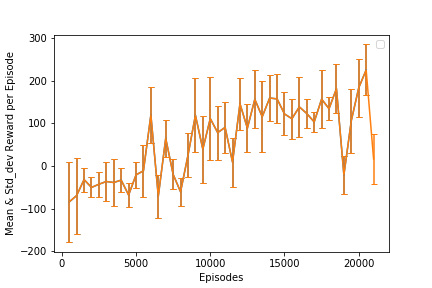
\includegraphics[scale=.73]{figures/A2C_LC_N=1_21.png}
				\end{center}
				\caption{A2C Algorithm N=1: learning curve. Wider critic network (30x30x30, relu activations for hidden layers, linear activation for output layer), critic lr = 0.001, actor lr = 0.001. First reached a mean reward of 225 after 20500 episodes.  } 	\label{2}%
			\end{figure}			
			  
			\begin{figure}[H]
				\begin{center} 
					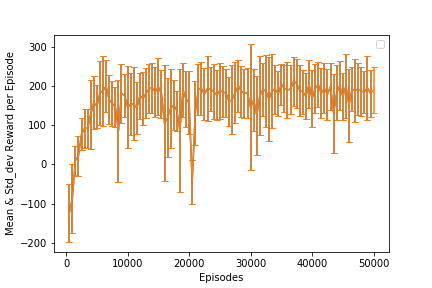
\includegraphics[scale=.73]{figures/A2C_LC_N=20_50.png}
				\end{center}
				\caption{A2C Algorithm N=20: learning curve. Actor and critic lr = 0.001. First reached a mean reward of 200 after 6500 episodes. } 	\label{3}%
			\end{figure}
			\begin{figure}[H]
				\begin{center} 
					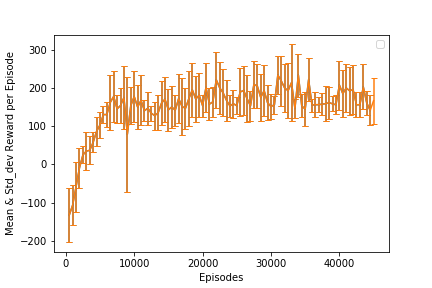
\includegraphics[scale=.73]{figures/A2C_LC_N=50_45.png}
				\end{center}
				\caption{A2C Algorithm N=50: learning curve. Actor and critic lr = 0.001. First reached a mean reward of 201 after 20500 episodes. } 	\label{4}%
			\end{figure}
        
			\begin{figure}[H]
				\begin{center} 
					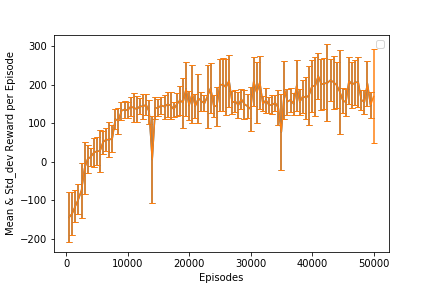
\includegraphics[scale=.73]{figures/A2C_LC_N=100_50.png}
				\end{center}
				\caption{A2C Algorithm N=100: learning curve. Actor lr=0.0008 and critic lr=0.001. First reached a mean reward of 200 after 25500 episodes.   } 	\label{5}%
			\end{figure}	
                
			\begin{figure}[H]
				\begin{center} 
					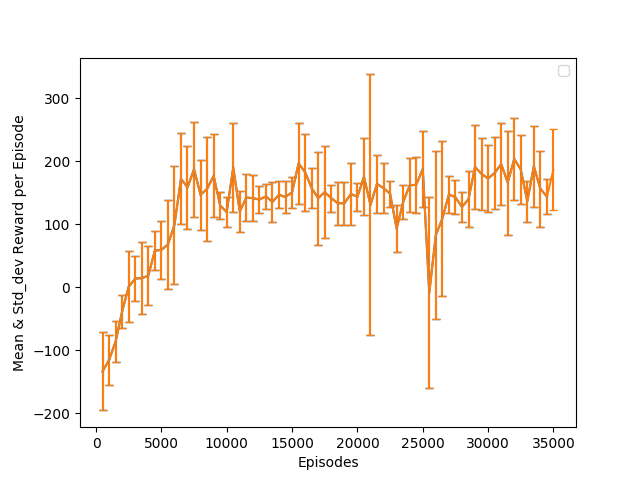
\includegraphics[scale=.73]{figures/A2C_LC_N=100_35.png}
				\end{center}
				\caption{A2C Algorithm N=100: 2nd learning curve showing slower convergence. Actor lr=0.001 and critic lr=0.001. First reached a mean reward of 204 after 32000 episodes.  } 	\label{6}%
			\end{figure}	  
				
		\item  REINFORCE and A2C comparisons:\\
		Compared to REINFORCE, n-steps A2Cs have much lower variance and accelerated learning, except for the case when n=1. As discussed, the REINFORCE algorithm without a baseline in its target introduces significant variance inherent to Monte Carlo sampling of episodic rewards. This hinders learning as rewards for optimal actions are not normalized and many more noisy gradient updates are required for convergence. The case of A2C with one-step critic introduce much more noise than n=20,50 and 100 A2Cs due to its greater dependence on bootstrapping from the learned critic network, which meant convergence was more difficult. 
		It seems that A2C algorithm with n=20, 50 and 100 learn faster than all other algorithms. Even though we were able to achieve a better performance for n=100 with an actor learning rate  of 0.0008 as seen in Figure \ref{5} above, we run A2C n=100 again for 35000 episodes with an actor lr=0.001 (Figure \ref{6} ) which is the same as the one used for A2C n=20 and n=50. This was done to make sure the comparison regarding speed of learning is fair enough since now the only difference between them is n, the number of steps for the critic's lookahead. (Note that we fix the random seed to $1234$ for all algorithms). 
		
		A2C n=20 was the fastest to reach a mean reward of 200 or greater. It achieved that after only 6500 episodes.
		A2C n=50 (50-steps return) comes second with 20500 episodes.  
		Third comes A2C n=100 with 32000 episodes. 
		Fourth comes Reinforce with 36000 episodes. However, for n=20, 50, and 100, these algorithms stably achieve 200 reward in the same range of episodes (between 20k and 31k).
		A2C n=1 was not able to achieve 200 with the same neural architecture for the critic as the other algorithms. However using a critic NN architecture that include 3 layers each with 30 units this time A2C n=1 achieved a reward of 225 after 20500 episodes similar to A2C n=50.
		Comparing figures \ref{3}, \ref{4} and \ref{6},
		it can be seen that A2C n=20 was quickest to reach 200 reward, then comes n=50 and finally n=100. More precisely, n=20 and n=50 had similar convergence, as both stably reached 200 reward around 20.5k episodes. \\\\
		We believe this is the case since 20-step and 50-step A2Cs struck the best balance for the LunarLander-v2 environment between bootstrapping using the learned critic value network and using the MC sampled episodic returns. 20-step A2C demonstrated wider variance in its training than 50-step, so 50-step A2C may arguably be preferrable. Generally, larger N for number of steps for A2C may be favored due to the longer nature of a typical successful episode of the LunarLander-v2 environment, in which the time to land is not greatly penalized and, instead, stable, complete deceleration of the lander agent within the landing zone is all that is required for reaching a score above 200. 
		
		
		
		
	\end{enumerate}
	
	
	
	
\end{document}
